\documentclass[10pt]{article}
\usepackage[top=1in,bottom=1in,left=0.5in,right=0.5in]{geometry}
\usepackage{graphicx}
\begin{document}

\title{Lab5 Timing Experiments : Observations and Inferences}
\author{ Sudipto Biswas, 110050048\\*
\\*
Sagar Jha, 110100024\\*
\\*
Mridul Garg, 110050030\\*
}
\date{\today}
\maketitle

\section{Introduction}
The Lab05 Timing experiments provided us with some very interesting plots relating and comparing loop time, step time, velocity update time, position update time and collision time.The purpose of this report is to list down all the distinct observations made regarding the \lq\lq Timing plots \rq\rq and to make an attempt to draw inferences from these observations.

\section{Error in the original ( de-patched ) Box2D code}
In the file b2Timer.cpp present in the common folder of Box2D package, there was an error initially, a logical error in the reset function. In the reset function defined for the linux version of the code, the variable $m\_start\_msec$ \ is defined as a long type variable. So when we calculate $m\_start\_msec$ from $m\_start\_usec$ by multiplying it with 0.001, the precision is lost. For Eg, if $m\_start\_usec$ is 489 which means $m\_start\_msec$ is 0.489 but as it is long, it will store 0, thus committing a huge error to the data. In the patched version we take care of this logical error by storing the time in a $timeval$ \ object, which in turn protects the data from such a loss of information and prevents it from subjection to error.

\section{Observations and Conclusions}
\subsection{Plot 01 : Step time and Total Loop time averaged over Reruns}
\begin{center}
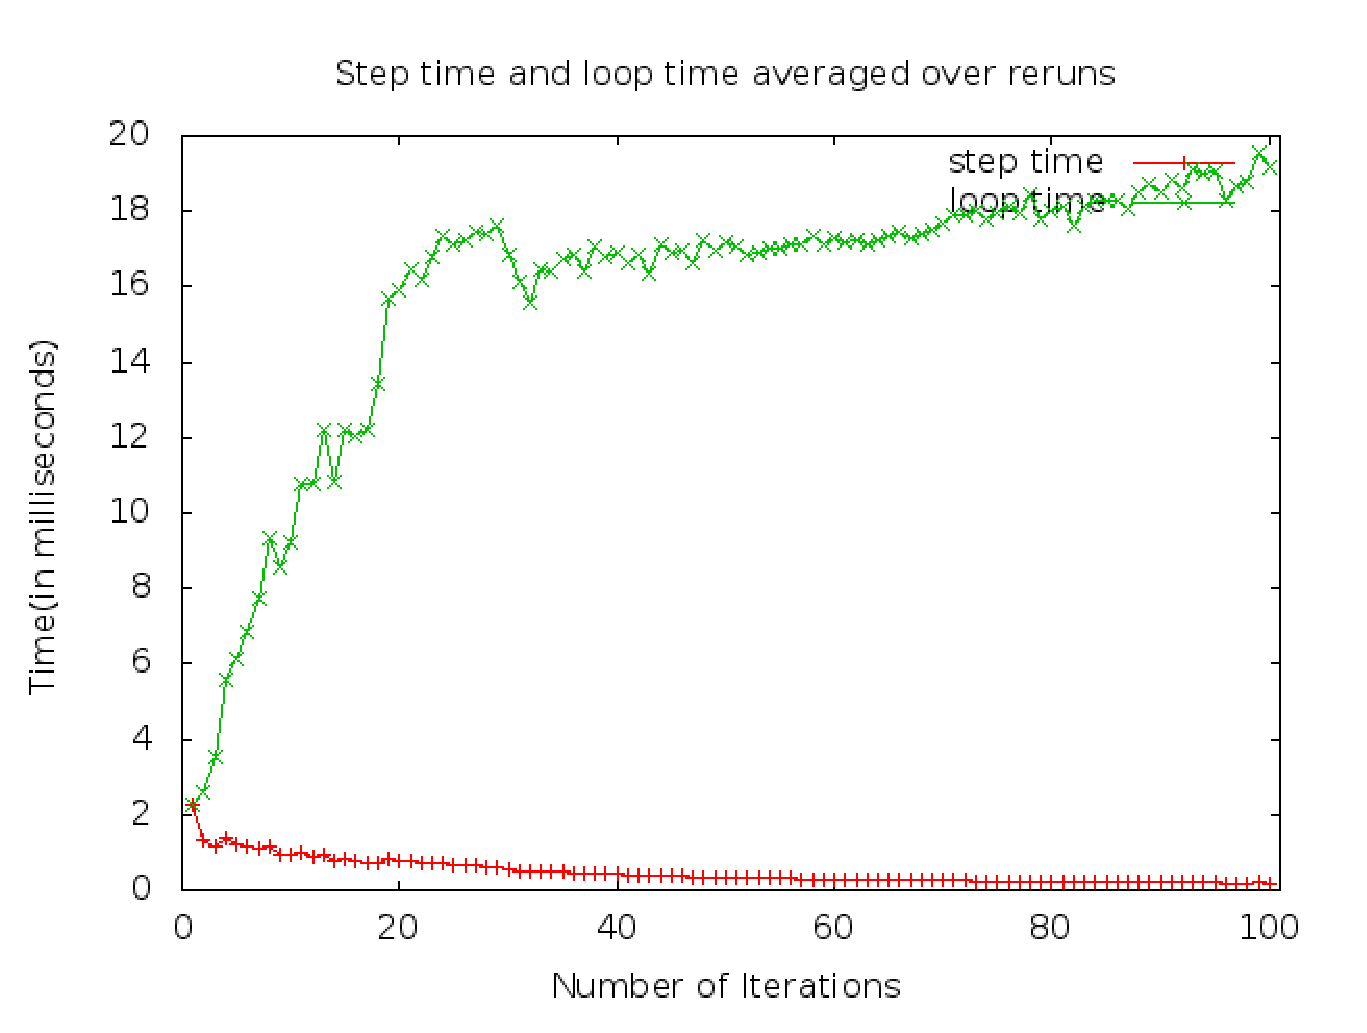
\includegraphics[scale=0.4]{plot1}
\end{center}
1.\ Loop time is greater than the Step time at all points except the first point where both are equal.
\\* 2.\ Total Loop time increases with the number of iterations whereas the Step time stays nearly constant or slightly decreases. \ \ This is because the loop executes iteration times but the step time is averaged over total iterations.
\subsection{Plot 02 : Step time, Velocity update time, Position update time and Collision time averaged over Reruns}
\begin{center}
\includegraphics[scale=0.4]{plot2}
\end{center}
1.\ Step time \textgreater \ velocity update time \textgreater \ position update time \textgreater \ collision time
\\*2.\ Each of these decrease slightly with the number of iterations
\\*3.\ The time taken to update velocity is highest becuase it involves more calculations than the other two.
\subsection{Plot 03 : Step time and Loop time averaged over Iterations}
\begin{center}
\includegraphics[scale=0.4]{plot3}
\end{center}
Since, there is no difference among the reruns, Step time and Loop time are very closely deviated about the average with the rerun number.
\subsection{Plot 04 : Step time, Velocity update time, Position update time and Collision time averaged over Iterations}
\begin{center}
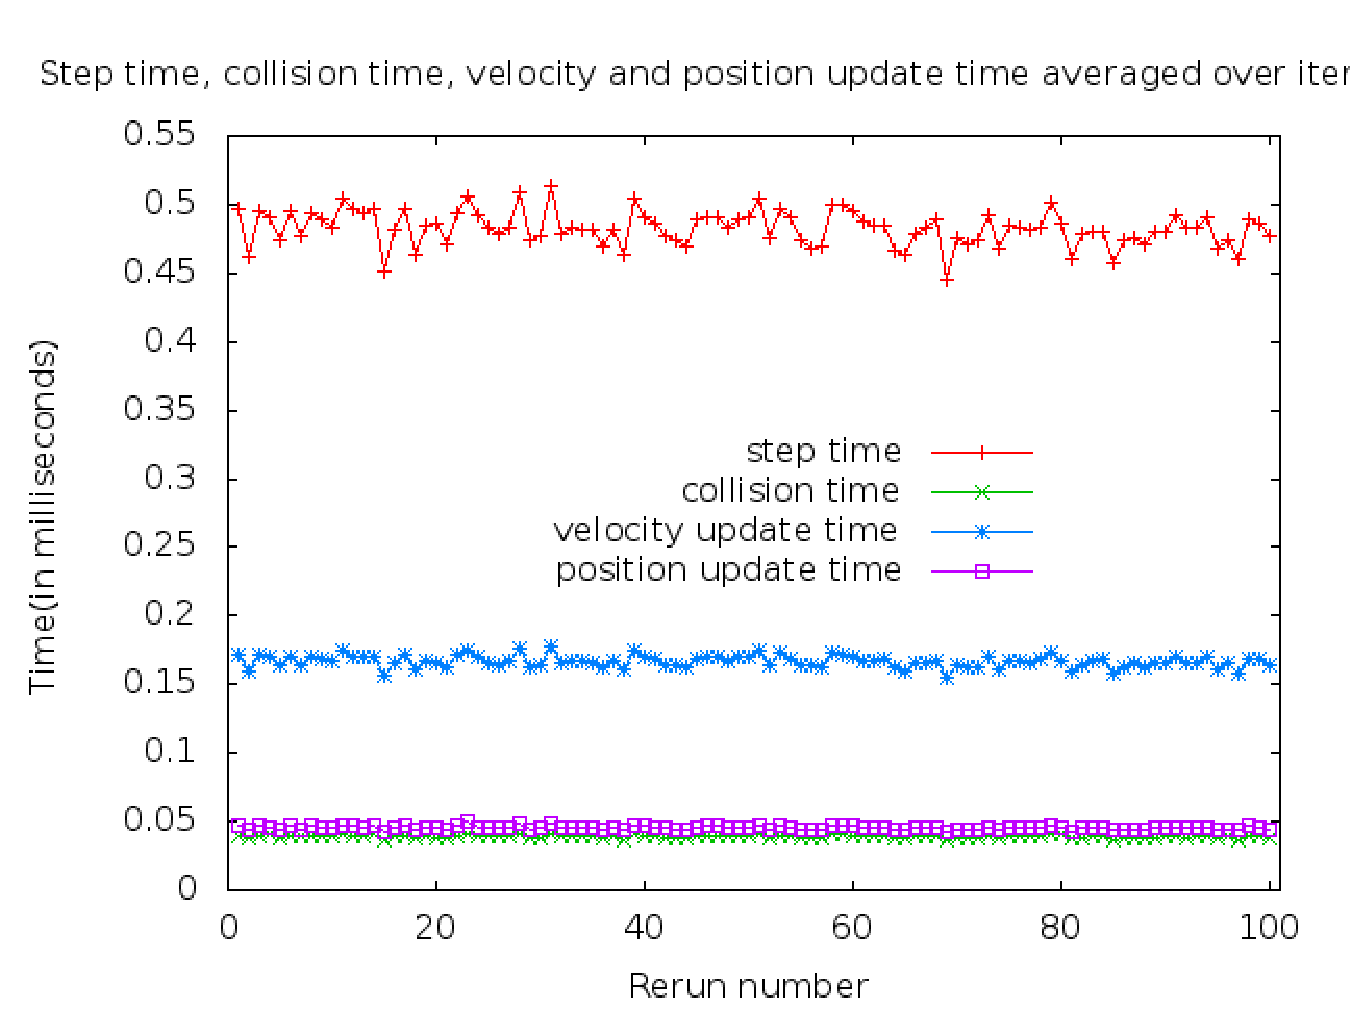
\includegraphics[scale=0.4]{plot4}
\end{center}
Same is the case with this plot of collision time, velocity update time and position update time. Like the previous plot, all of them are slightly deviated about their respective averages with the rerun number.
\subsection{Plot 05 : Deviation in all the Time measurements}
\begin{center}
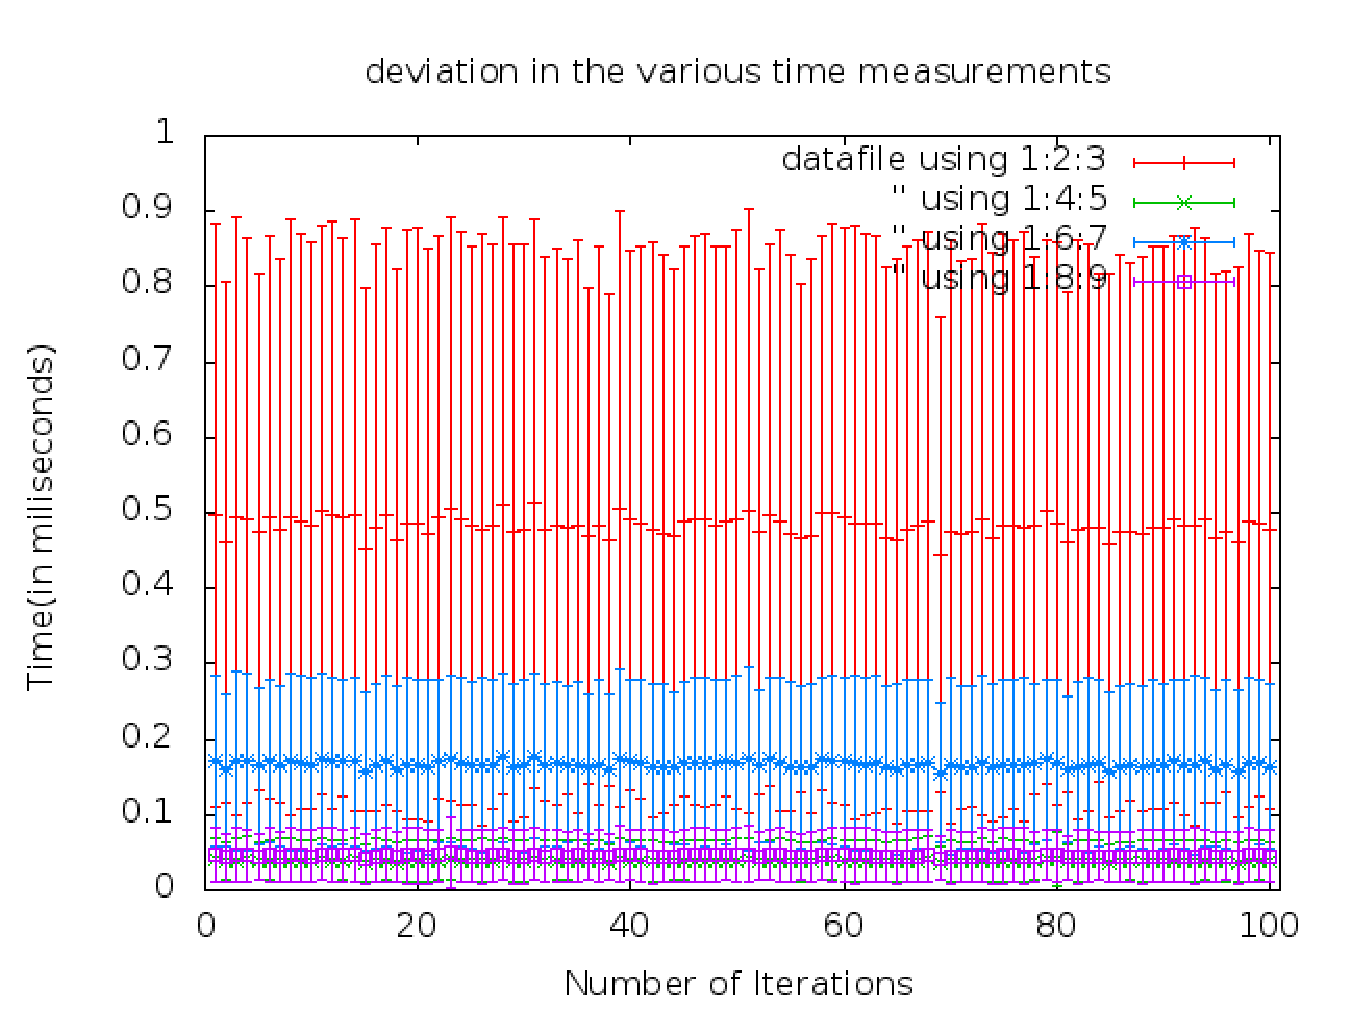
\includegraphics[scale=0.4]{plot5}
\end{center}
1.\ Deviation of Step time \textgreater \ Velocity update time \textgreater \ Position update time \textgreater \ Collision time
\\*2.\ This together with the second plot shows that the percentage deviation of all the three is nearly equal.
\subsection{Plot 06 : Step time and Loop time averaged over Reruns for no heavy processes and many CPU heavy processes}
\begin{center}
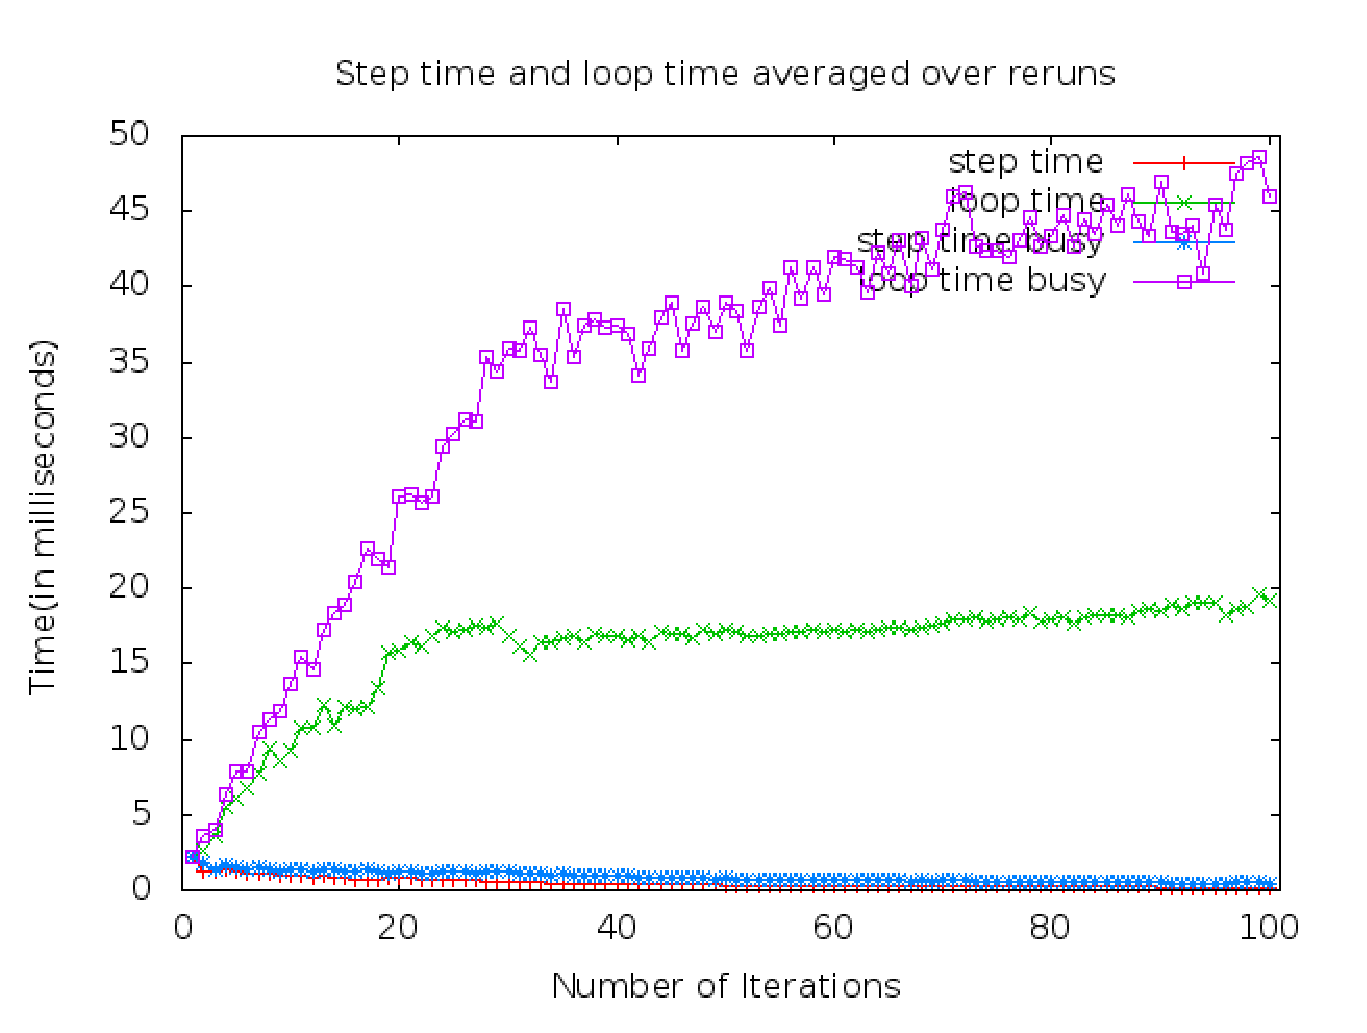
\includegraphics[scale=0.4]{compare1}
\end{center}
\subsection{Plot 07 : Step time, Velocity update time, Position update time and Collision time averaged over Reruns for no heavy processes and many CPU heavy processes}
\begin{center}
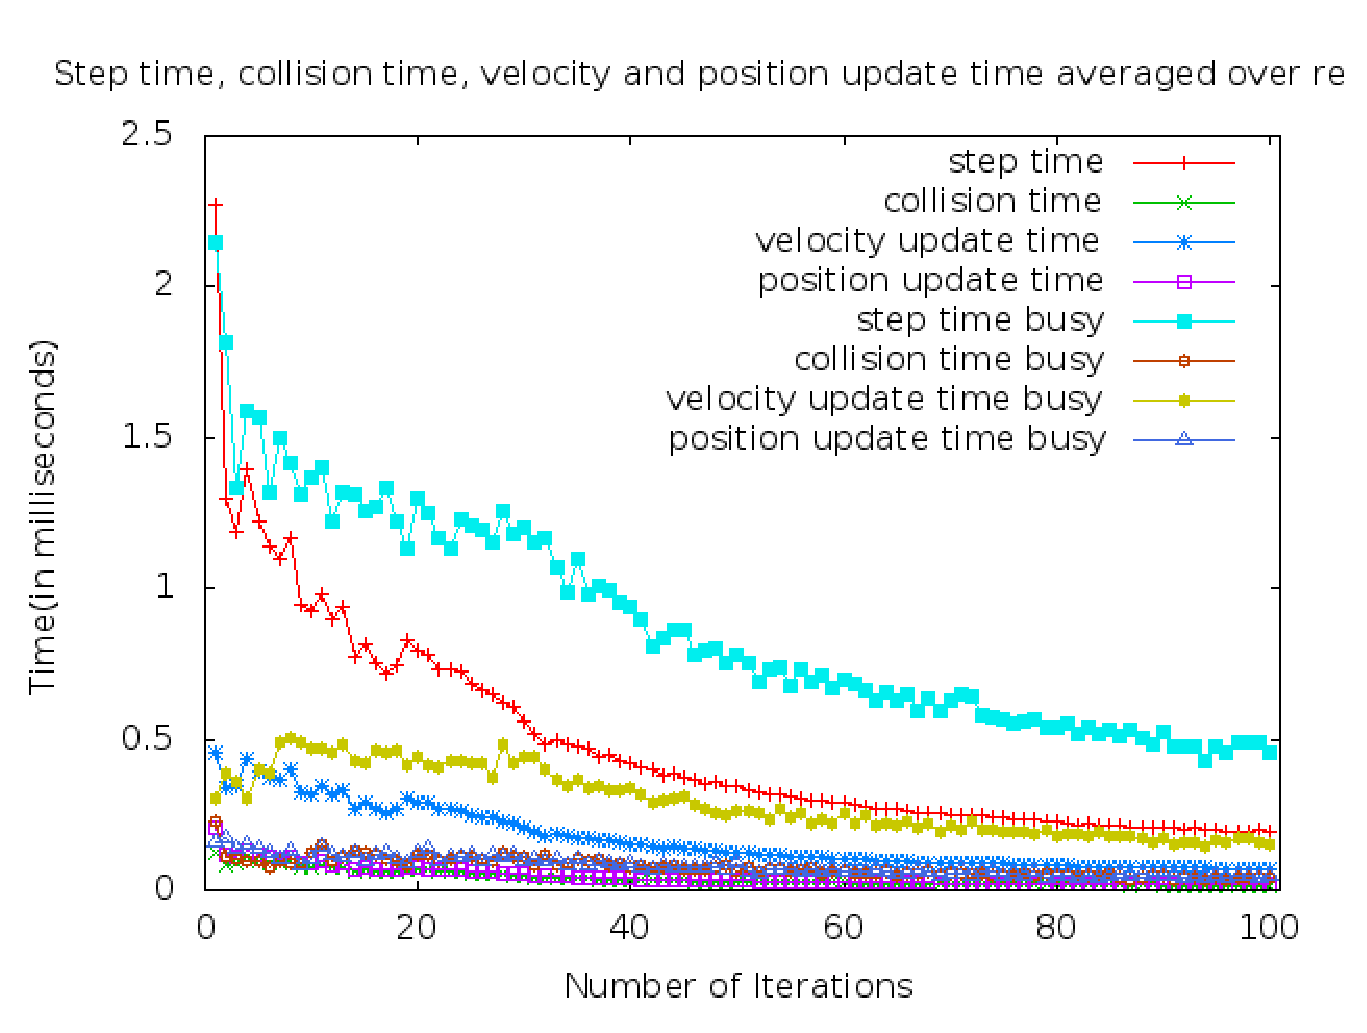
\includegraphics[scale=0.4]{compare2}
\end{center}
We can see from the above two plots that the loop time, step time and times for velocity, position and collision updates are significantly higher in the case when many CPU heavy processes are running as compared to the case when the CPU is occupied only by our executable.
\section{Profiling the Code : Observations and Conclusions}
For our code, \textbf{gprof} has been used to profile the Lab05 code with number of iterations and reruns. Iterations and rerun values were varied from 1000 to 10000 over 1000 steps. Profiled data was collected for executable running in \textbf{debug} and \textbf{release} mode. This report is an attempt to explain the observations made from the output.
\\*From the Graph of Function calls, we can infer that release mode of the executable is optimised as its function-call graph structure has no function call arrows which means that function calls are reduced by a significant amouont. On the other hand, the graph of debug mode shows the actual function calls without any optimisation from the compiler.
\\*The release mode uses the -O3 flag while compiling in unlike the debug mode. -Ox is the class of g++ flags which enables the compiler to optimize the code. 

\subsection{Release Mode}
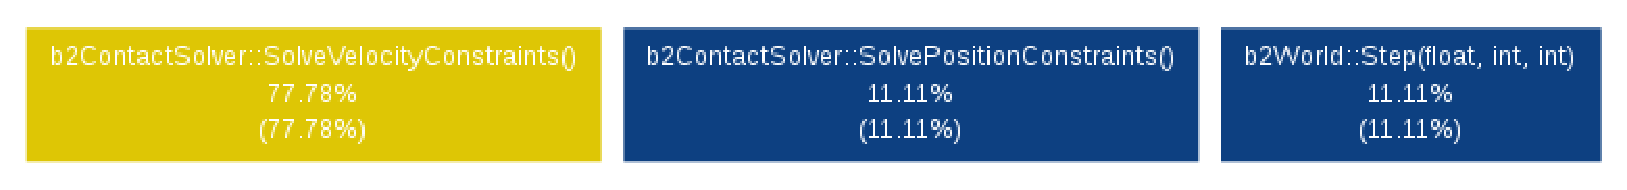
\includegraphics[scale=0.15]{release}
\begin{center}
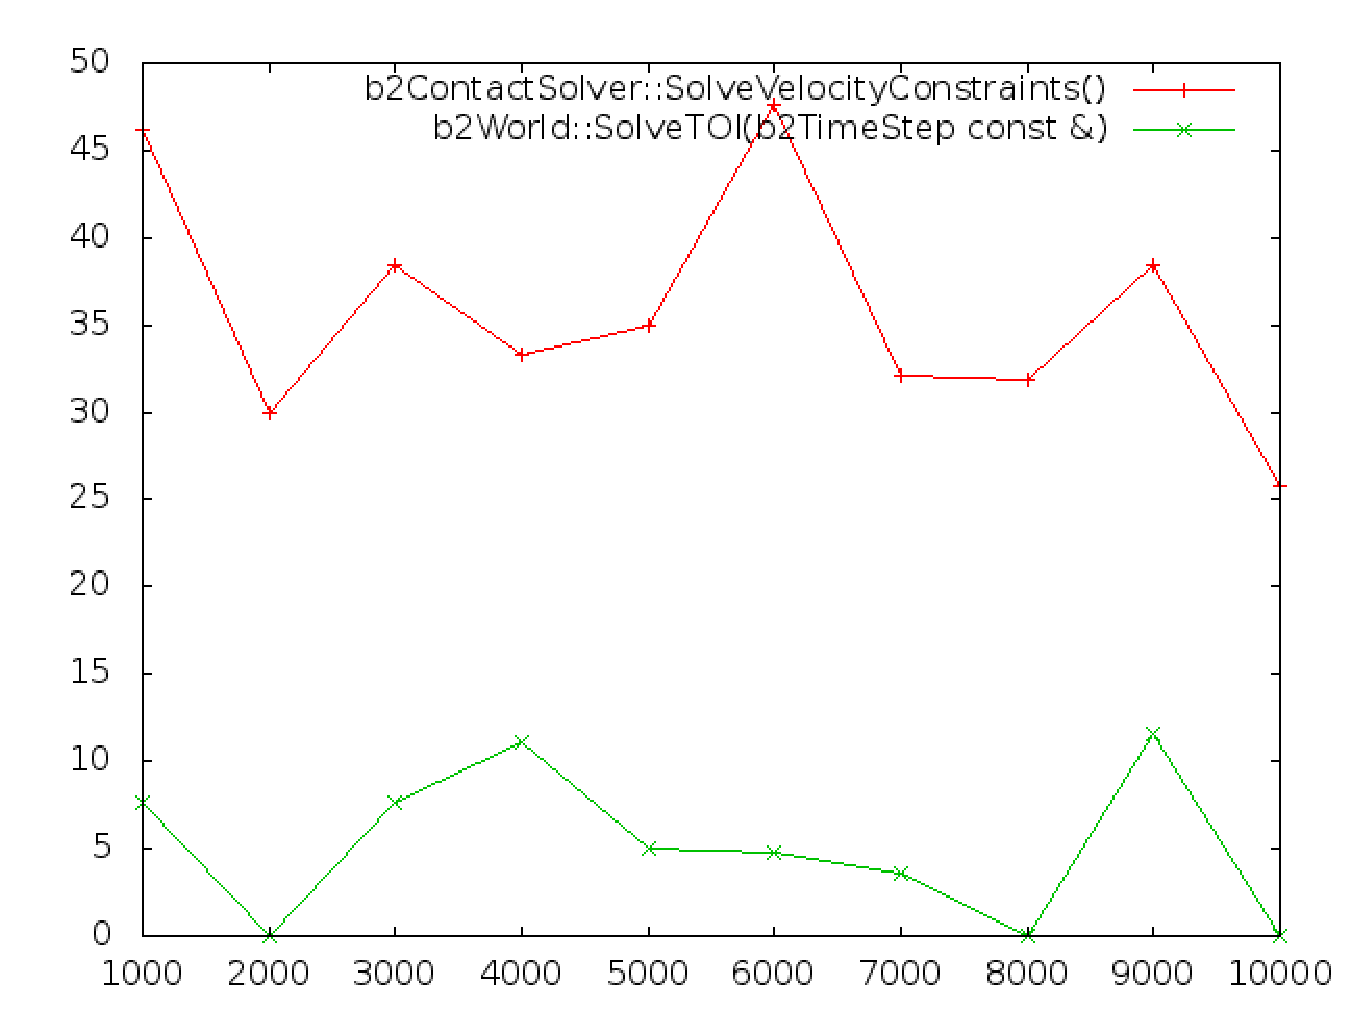
\includegraphics[scale=0.4]{release1}
\end{center}
Observing the .dat file for release mode, namely $g06\_release\_prof.dat$ in this case, we infer that in most cases, $b2ContactSolver::SolveVelocityConstraints()$ function takes most of the execution time.
\subsection{Debug Mode}
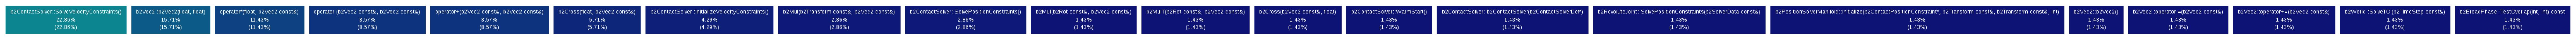
\includegraphics[scale=0.075]{debug}
\begin{center}
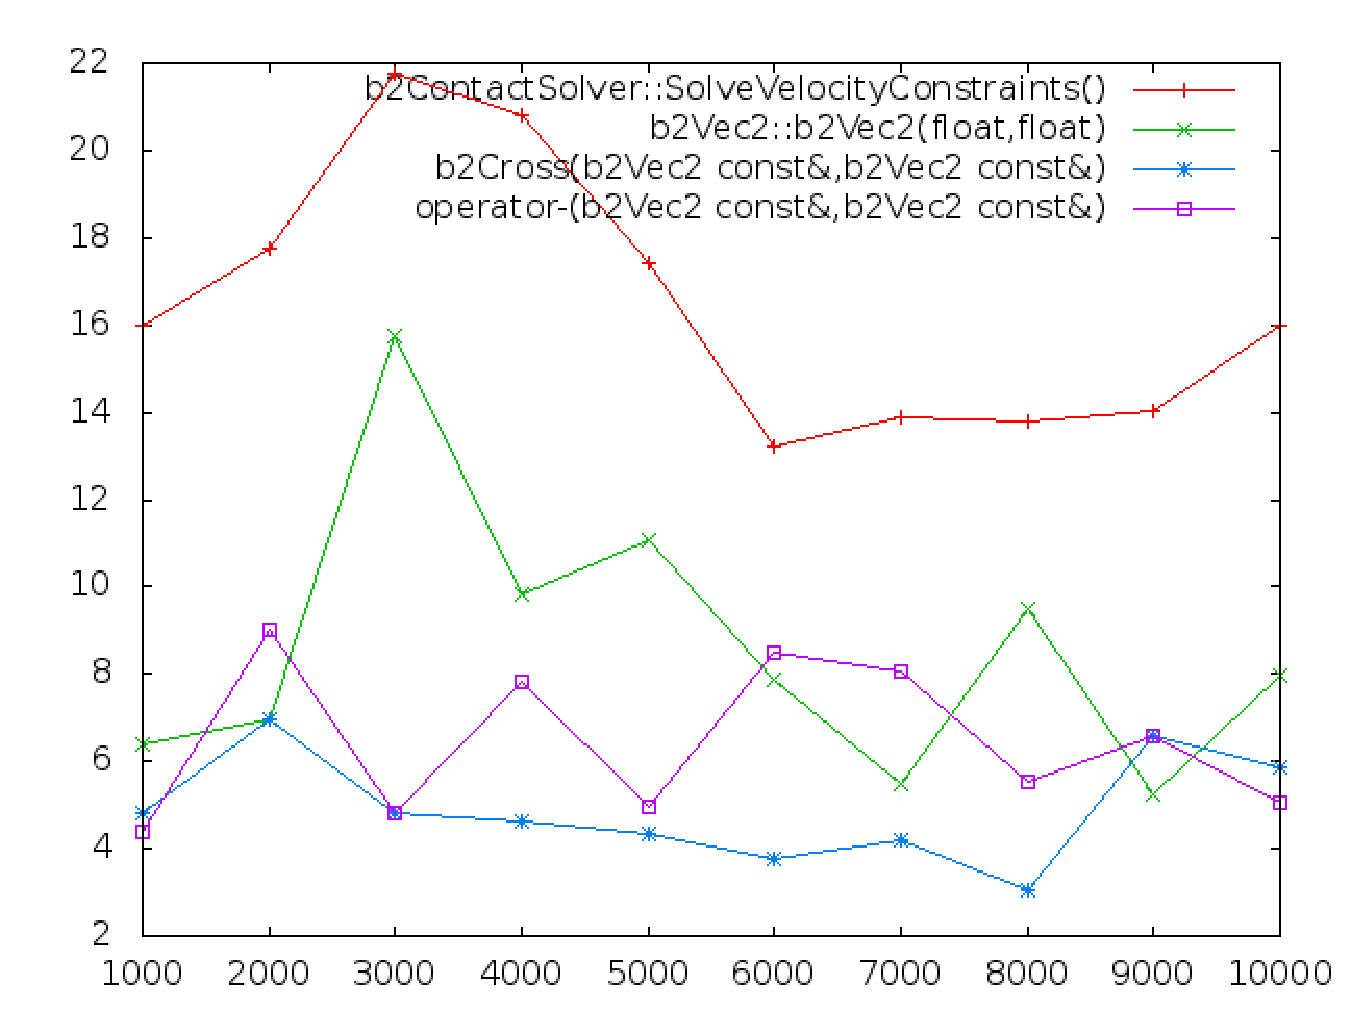
\includegraphics[scale=0.4]{debug1}
\end{center}
In case of Debug Mode, observing the .dat file, namely $g06\_debug\_prof.dat$, we infer that functions like operator*(), opertor-(), b2Vec2(float, float) etc. also consume execution time approximately distributed equally among them along with $b2ContactSolver::SolveVelocityConstraints()$. These functions did not take significant share of execution time in release mode. The reason being debug mode doen not optimise the code. Thus, as a result other functions which otherwise would have taken less time in release mode are now consuming significant time.

\end{document}
